\chapter{Test Cases}
\label{ch:testcases}
Test Cases were developed in this study for the purpose of comparing and validating different drill string models.  The Test Cases are meant to be general and provide a reliable means of cross-checking and comparing the performances of various models, not just those specific to the current study.  As such, the key parameters, borehole design, and other information required to reproduce the Test Cases is provided.

\section{Recommended Procedures for Developing Test Cases}
\notfinished{}
When working with various friction models, it becomes vital to identify parameters that result in similar frictional behaviors. Ensuring accurate unit conversion is also a key aspect of this process. The parameters for the friction models are static, dynamic and critical velocity. Generally, the static and dynamic friction factors can be equated across different models, while special attention is required to align the critical velocity with the desired frictional behavior. In the context of modeling torsional dynamics, if the critical velocities of two different models are provided in different units such as meters per second ($m/s$) and revolutions per minute ($RPM$), unit compatibility must first be established for meaningful comparison. Converting $m/s$ to $RPM$ can be achieved by \equationname~\ref{velocity_conversion}.
\begin{equation}\label{velocity_conversion}
  N_{(rpm)}=v_{(m/s)}\frac{60}{2\pi}*r_o
\end{equation}
where $N$ and $v$ are angular velocity expressed in $RPM$, and $m/s$, respectively, and $r_o$ is outer radius of the drill pipe. For instance, considering Test Case 2 with a critical velocity of 0.03 $m/s$ and a drill string radius of 0.075 $m$, the critical velocity can be converted to 4$RPM$. After matching the units, the critical angular velocity of the model, which is for the comparison, can be decided by comparing the frictional force with respect to angular velocity.

\figurename~\ref{figure:stribeck_coulomb_friction} shows the example of comparison between Coulomb and Stribeck friction model with different critical velocity of Coulomb model with 4$RPM$ angular critical velocity for Stribeck model. In this project, we deliberately designate an angular velocity of 10 $RPM$ for the Coulomb model, chosen as a more extreme scenario. This choice allows us to align the exponentially decreasing component of the Stribeck model with the static friction inherent in the Coulomb friction model. However, it is important to note that additional tests involving different angular velocities have been performed and are included in the appendix chapter for comprehensive analysis.\reviewcomment{If not added, modify}.
\begin{figure}
  \centering
  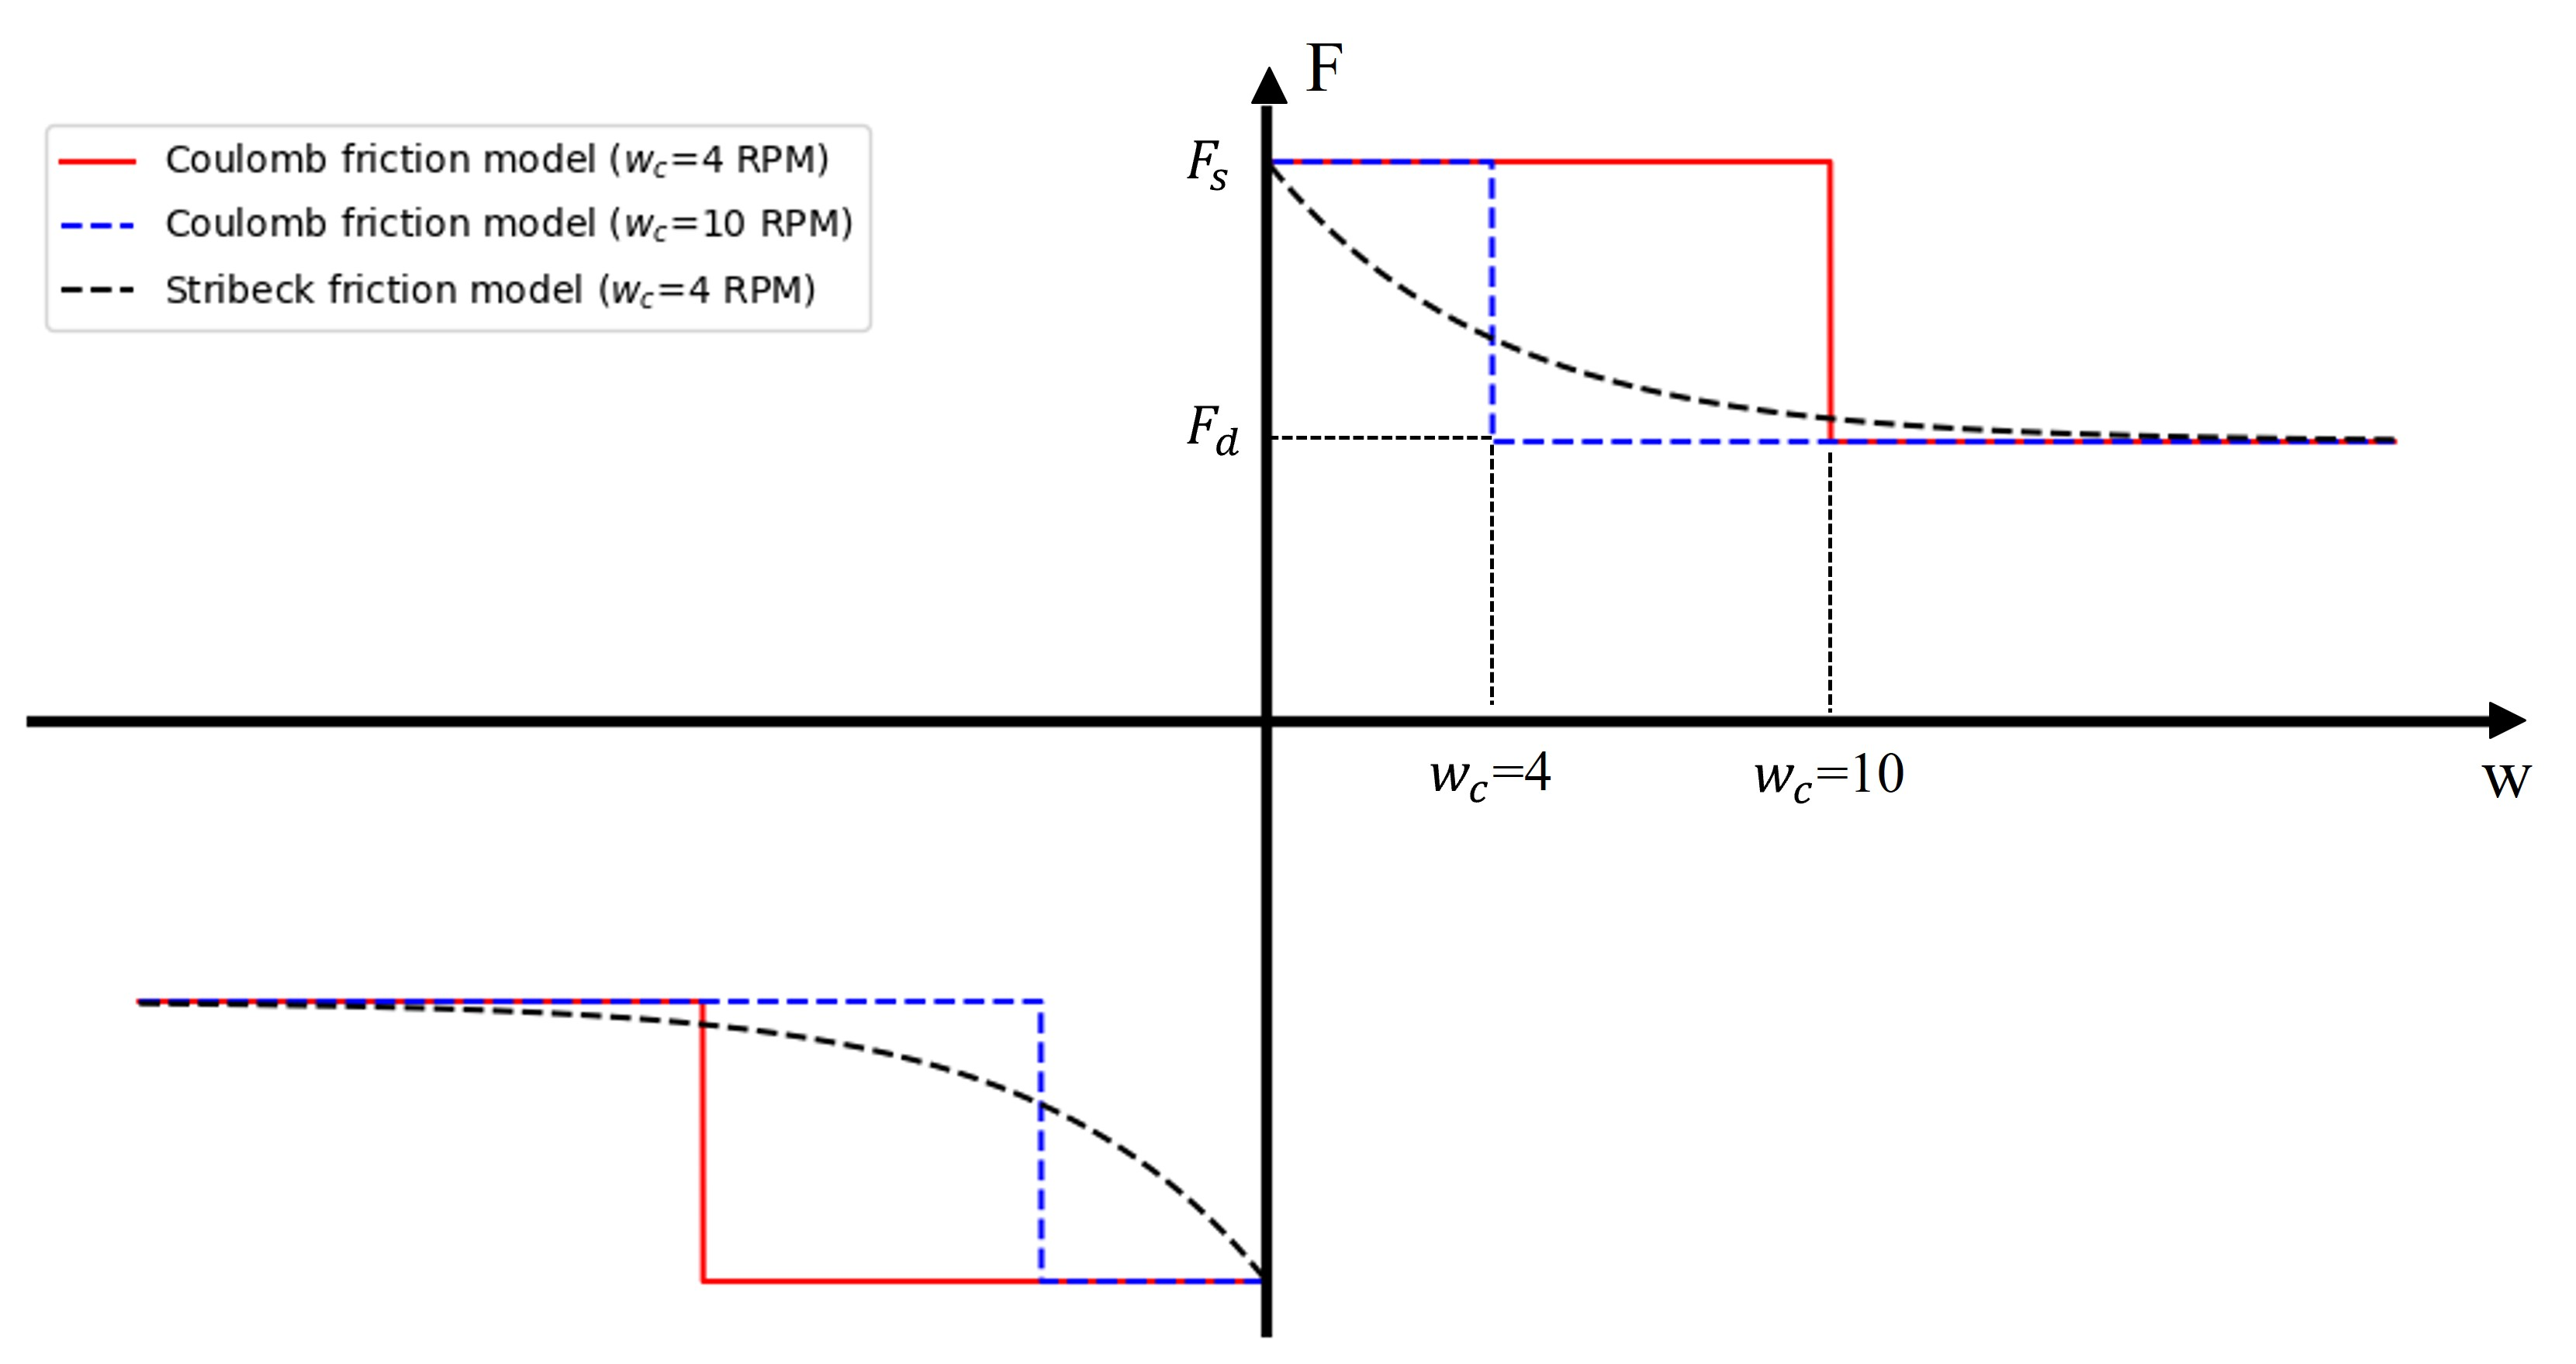
\includegraphics[width=5in]{Stribeck_Coulomb_friction}
  \caption[Comparison between Coulomb and Stribeck friction model]{Comparison between Coulomb and Stribeck friction models assuming same normal force at the drill string wellbore contact. Stribeck model with a critical angular velocity of 2 $RPM$ and Coulomb friction model with a critical angular velocity of 4$RPM$ and 10$RPM$ is compared. $F_s$ and $F_d$ represents static and dynamic friction, respectively, and $w$ represents the angular velocity.}\label{figure:stribeck_coulomb_friction}
\end{figure}

\section{Overview of Test Cases}
In total, six Test Cases are presented. Test Cases 1 and 3 encompass scenarios involve vertical wells, with the distinction being the presence of BHA components. Similarly, Test Cases 2 and 4 are the deviated well scenarios with a 60\textdegree{} inclination angle. The difference between Test Cases 2 and 4 is the exitance of BHA components. In addition, to analyze the effect of frictional factors, Test Cases 2 and 4 are further divided into \emph{a} and \emph{b} subcases (2a, 2b, 4a, 4b). The friction factors are tested in the deviated wells because in a vertical well gravity does not create contact force (normal force). All the current Test Cases are for off-bottom scenarios. \tablename~\ref{Test_case_summary} summarizes the scenarios for each Test Case.
\begin{table}
  \centering
  \begin{tabular}{|c|c|c|c|c|c|c|}
    \hline
    \tablecolumnheadervlinesone{Test Case} & \tablecolumnheadervlinestwo{Well Type} & \tablecolumnheadervlinestwo{Static} & \tablecolumnheadervlinestwo{Dynamic} & \tablecolumnheadervlinestwo{Viscous} & \tablecolumnheadervlinestwo{BHA} \\[-7pt]
                                           &                                        & \tablecolumnheadervlinestwo{FF}     & \tablecolumnheadervlinestwo{FF}      & \tablecolumnheadervlinestwo{Damping} & \\
    \hline
    Test Case 1 & Vertical & 0 & 0 & 0 & N \\
    \hline
    Test Case 2a & Deviated (60\textdegree{}) & 0.5 & 0.5 & 0 & N \\
    \hline
    Test Case 2b & Deviated (60\textdegree{}) & 0.5 & 0.25 & 0 & N \\
    \hline
    Test Case 3 & Vertical & 0 & 0 & 0 & Y \\
    \hline
    Test Case 4a & Deviated (60\textdegree{}) & 0.5 & 0.5 & 0 & Y \\
    \hline
    Test Case 4b & Deviated (60\textdegree{}) & 0.5 & 0.25 & 0 & Y \\
    \hline
  \end{tabular}
  \caption[Scenarios of the defined Test Cases]{Scenarios of the defined Test Cases.}
  \label{Test_case_summary}
\end{table}
Additionally, the viscous damping is neglected for the simplicity of the tests in this project, but it can be included in future studies.  The tests were conducted by assuming the top drive velocity to be increased from 0 $RPM$ to 40 $RPM$ at 1 second and maintained the velocity for the rest of the time. The top drive set velocity is shown in \figurename~\ref{figure_topdrive_VSP}
\begin{figure}
  \centering
  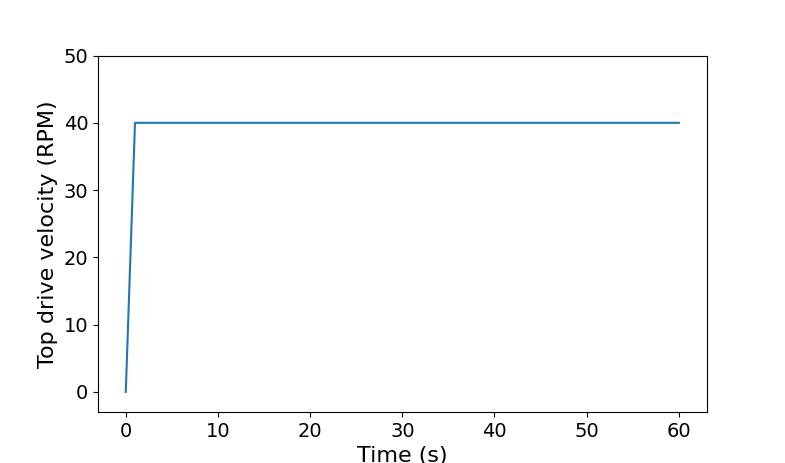
\includegraphics[width=3.75in]{TopdriveVSP}
  \caption[Top drive velocity profile for the Test Cases]{Top drive velocity profile for the Test Cases.}\label{figure_topdrive_VSP}
\end{figure}

\section{Terminology}
\subsection{With BHA vs Without BHA}
The Test Cases enable comparing drilling scenarios with and without the BHA components. This allows the influence of the BHA to be examined for each model by comparing the two cases.

\begin{definition}{Without BHA}
Analysis with a single drill pipe configuration to maintain simplicity and establish a baseline. This configuration represents the most straightforward drilling arrangement, with a solitary pipe running from the surface to the drill bit. In this case, the weight and diameter of the entire drill pipe are uniform and tool joints are ignored.
\end{definition}
\begin{definition}{With BHA}
This case is based on the Without BHA case with the notable difference that a BHA is added.  The weight and diameter of the drill pipe is are uniform, however, the BHA's distinct parameters are considered in the analysis.  Tool joints are ignored.
\end{definition}

%In the next subsection we will explore additional configurations with varying BHA designs and properties to further investigate their influence on drilling efficiency and performance. These test cases will enable us to optimize drilling operations and develop a comprehensive understanding of how the presence or absence of the BHA affects the system's behavior.

\subsection{Friction Factors}
Many drill string models take into account both static and dynamic friction between the drill string and wellbore. The friction factors (FF) will affect the drill string motion in deviated well, since the interaction between the drill string and the wellbore wall becomes complex.\wording{}  Therefore, to gain insights into the impact of friction factors on drilling dynamics, a detailed investigation is warranted.\wording{}
%but the disparity in FF values is expected to be more pronounced in inclined wells compared to vertical ones.
%This results in differing frictional forces acting on the drill string as it traverses the wellbore. As a consequence, the FF values play a crucial role in affecting the drilling performance and behavior.

\begin{definition}{Zero FF}
Tests conducted with the friction factors set to zero.
\end{definition}
\begin{definition}{Same FF}
Tests conducted with the same value of static and dynamic friction.
\end{definition}
\begin{definition}{Different FF}
Tests conducted with different values of static and dynamic friction.
\end{definition}




\section{Test Case 1 - Vertical Well Without BHA - Zero FF}
The model parameters and schematic of the wellbore surveys and drill string components for Test Case 1 are shown in \tablename~\ref{table_verticalwell_input} and \figurename~\ref{figure_verticalwell}. The model were tested with vertical well with MD of 2000 $m$ and bit depth of 1800 $m$. The ExxonMobil model and Matlab ver.\ A-S model uses metric units while Python ver.\ A-S model uses imperial units. For the future convenience, the tables in this chapter contains both imperial and metric units.

\begin{figure}
  \centering
  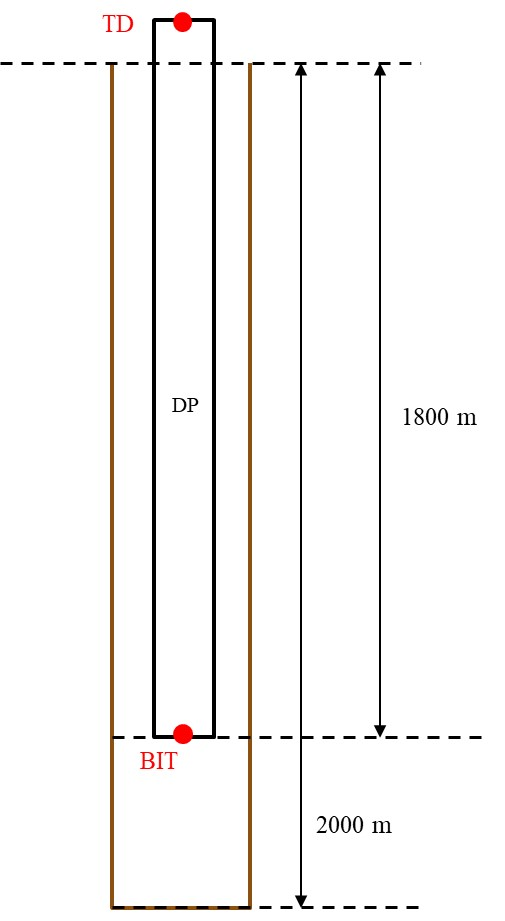
\includegraphics[width=1.5in]{VerticalWellConfig}
  \caption[Schematic of wellbore and drill string for Test Case1]{Schematic of wellbore and drill string for Test Case1}\label{figure_verticalwell}
\end{figure}


\begin{table}
    \centering
	\begin{testcasetable}
		$\rho$ & 490.6 $lb/ft^3$ & 7850 $kg/m^3$ & Drill pipe density \\
		\hline
		$G_{dp}$ & 1.67$\cdot$10$^{9}$ $lbf/ft^2$ & 7.99$\cdot$10$^{10}$ $Pa$  & Shear modulus \\
		\hline
		$OD_{dp}$ & 5.88 $in$ & 0.15 $m$ & Drill pipe outer diameter \\
		\hline
		$ID_{dp}$ & 5.00 $in$ & 0.127 $m$ & Drill pipe inner diameter  \\
		\hline
	\end{testcasetable}
	\caption[Input parameters for Test Case 1]{Input parameters for Test Case 1, a vertical well without BHA components.}\label{table_verticalwell_input}
\end{table}

\section{Test Case 2 - Deviated Well Without BHA}
\subsection{Test Case 2a - Same FF Values}
The models were tested with deviated well with simple configuration of drill string. The MD of the well is 4000 $m$ with 60$^{\circ}$ inclination from KOP of 1500 $m$. The drill bit is off-bottom where located at 2500 $m$ depth. The Schematic view of wellbore and drill string are depicted in \figurename~\ref{figure_wellconfig_inclined}. The static and dynamic friction factors were set to be the same as 0.5. The parameters for the test are summarized in \tablename~\ref{table_Inclinedwell_2a_input}.

\begin{figure}
  \centering
  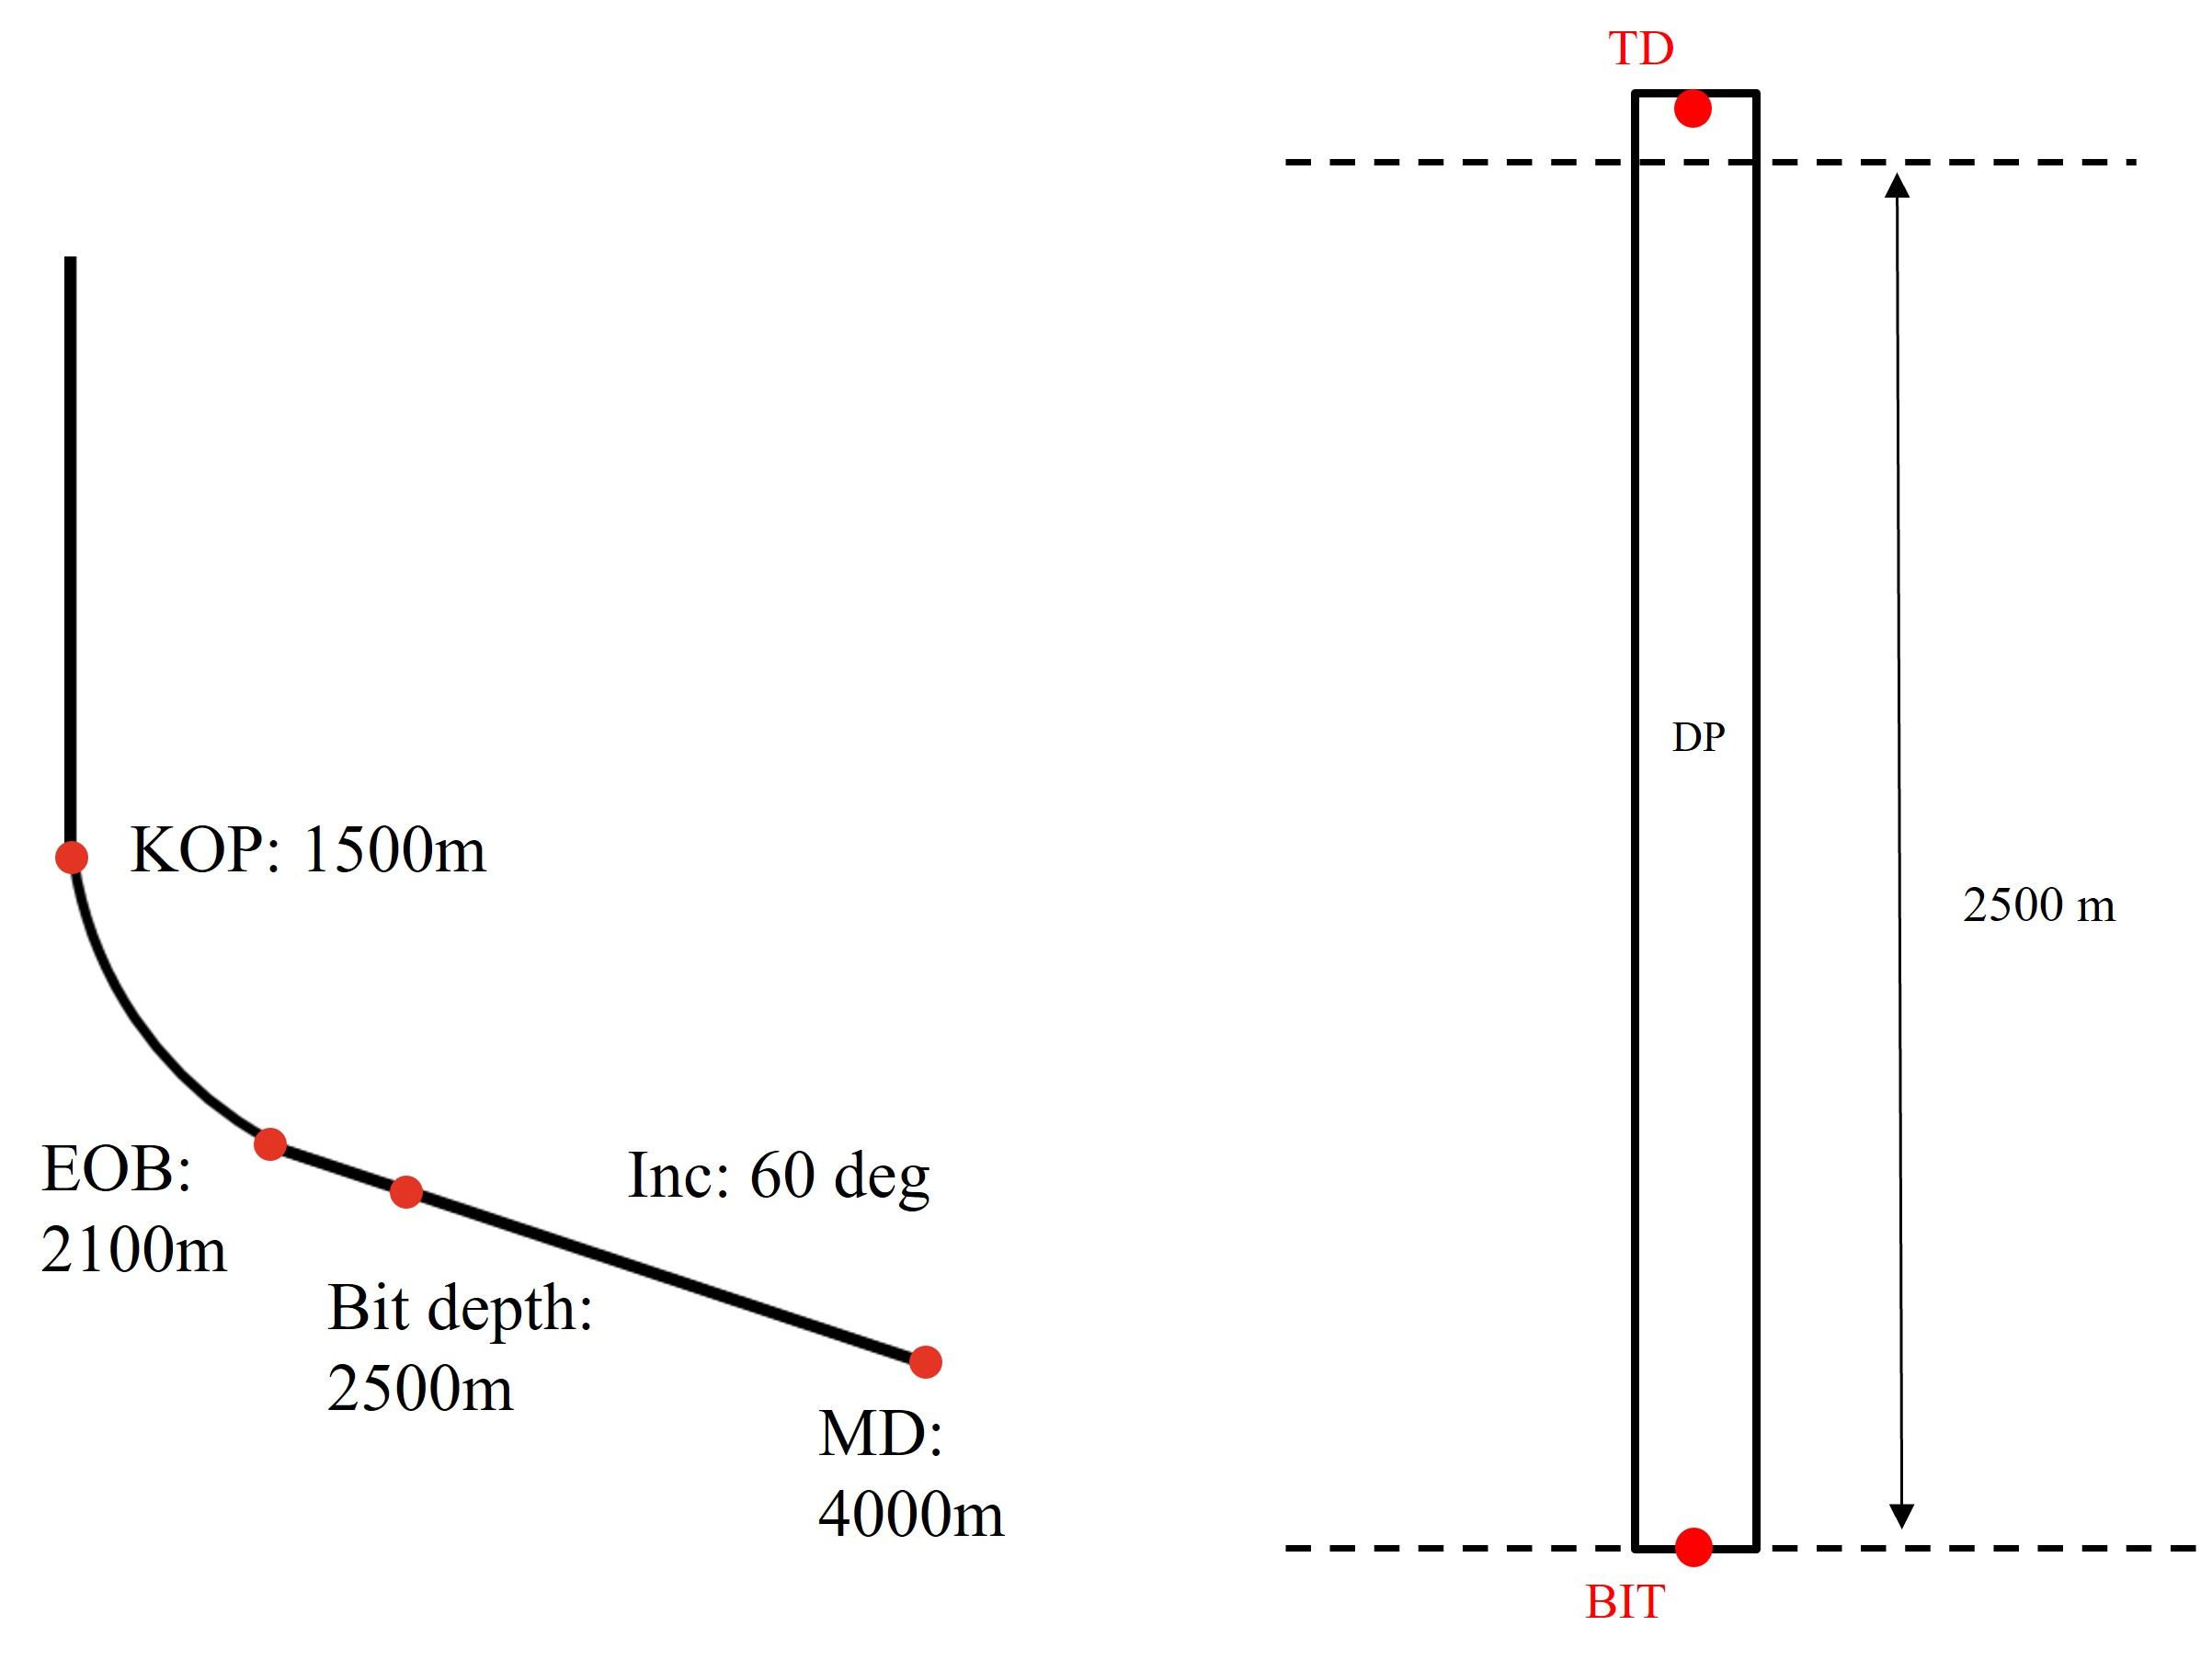
\includegraphics[width=4in]{InclinedWellConfig}
  \caption[Schematic of Test Case 2]{Schematic of wellbore and drill string for Test Case 2.}\label{figure_wellconfig_inclined}
\end{figure}

\begin{table}
    \centering
	\begin{testcasetable}
		$OD_{dp}$ & 5.88 $in$ & 0.15 $m$ & Drill pipe outer diameter\\
		\hline
		$ID_{dp}$ & 5.00 $in$ & 0.127 $m$ & Drill pipe inner diameter  \\
		\hline
		$\rho_{dp}$ & 490.6 $lb/ft^3$ & 7850 $kg/m^3$ & Drill pipe density \\
		\hline
		$G_{dp}$ & 1.27$\cdot$10$^{9}$ $lb/ft^2$ & 6.10$\cdot$10$^{10}$ $Pa$ & Drill pipe shear modulus\\
		\hline
		$\mu_{s}$ & 0.5 & 0.5 & Static friction factor\\
		\hline
		$\mu_{d}$ & 0.5 & 0.5 & Dynamic friction factor\\
		\hline
		$w_c$ & 10 $RPM$ & 10 $RPM$ & Cut-off angular velocity\\
		\hline
		$\theta$ & 60$^{\circ}$ & 60$^{\circ}$ & Inclination\\
		\hline
	\end{testcasetable}
	\caption[Input parameters for Test Case 2a]{Input parameters for Test Case 2a, a deviated well without BHA components and has the same dynamic and static friction factor values.}\label{table_Inclinedwell_2a_input}
\end{table}

\subsection{Test Case 2b - Different FF Values}
The models were tested with the exact same configuration with Test Case 2a, except different values of static and dynamic friction factor values. The following \tablename~\ref{table_Inclinedwell_2b_input} summarizes the input parameters.

\begin{table}
	\centering
	\begin{testcasetable}
		$OD_{dp}$ & 5.88 $in$ & 0.15 $m$ & Drill pipe outer diameter\\
		\hline
		$ID_{dp}$ & 5.00 $in$ & 0.127 $m$ & Drill pipe inner diameter  \\
		\hline
		$\rho_{dp}$ & 490.6 $lb/ft^3$ & 7850 $kg/m^3$ & Drill pipe density \\
		\hline
		$G_{dp}$ & 1.27$\cdot$10$^{9}$ $lb/ft^2$ & 6.10$\cdot$10$^{10}$ $Pa$ & Drill pipe shear modulus\\
		\hline
		$\mu_{s}$ & 0.5 & 0.5 & Static friction factor\\
		\hline
		$\mu_{d}$ & 0.25 & 0.25 & Dynamic friction factor\\
		\hline
		$w_c$ & 10 $RPM$ & 10 $RPM$ & Cut-off angular velocity\\
		\hline
		$\theta$ & 60$^{\circ}$ & 60$^{\circ}$ & Inclination\\
		\hline
	\end{testcasetable}
	\caption[Input parameters for Test Case 2b]{Input parameters for Test Case 2b, a deviated well without BHA components and has different dynamic and static friction factor values.}\label{table_Inclinedwell_2b_input}
\end{table}

\section{Test Case 3 - Vertical Well with BHA - Zero FF}
In this specific scenario, an BHA components were added to the drill string. The BHA introduced extra components, resulting in an increase in both the weight and size of the drill string. However, the well survey data for the vertical well remained the same, which well design, depicted in \figurename~\ref{Vert_well_conf_BHA}, remained unchanged. The specific input parameters can be found in the \tablename~\ref{Input Parameters TC3}.

\begin{figure}
  \centering
  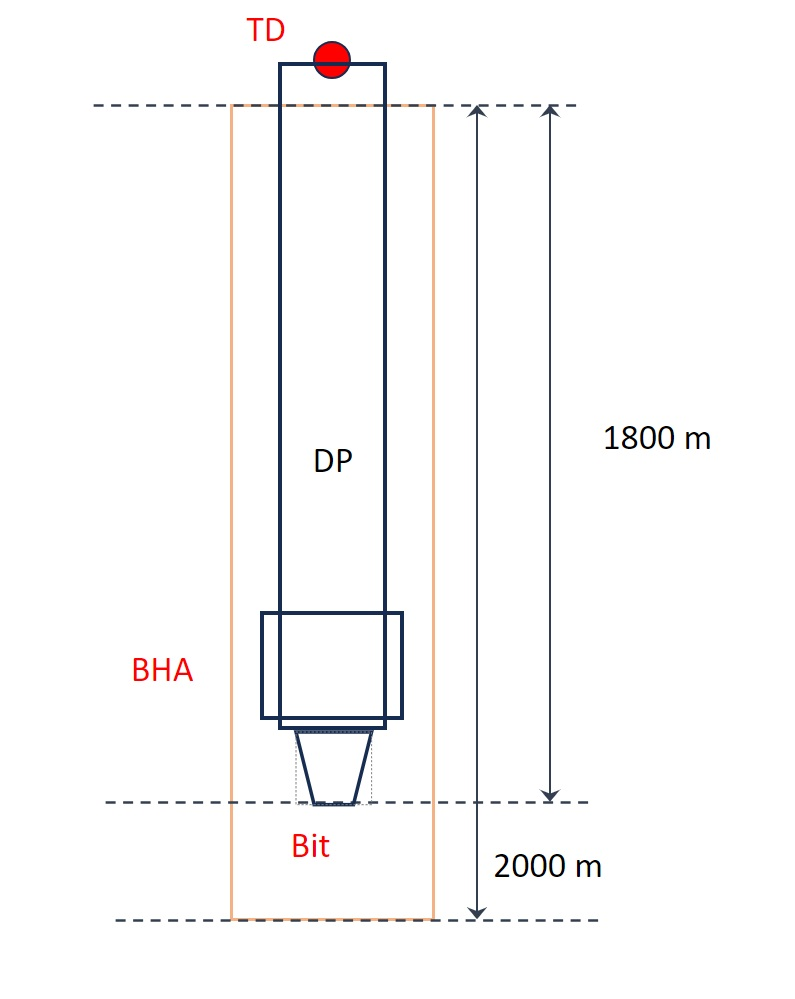
\includegraphics[width=2in]{VerticalWellConfigBHA}
  \caption[Schematic of well and drill string for model comparison]{Schematic of well and drill string for model comparison.}\label{Vert_well_conf_BHA}
\end{figure}


\begin{table}
    \centering
	\begin{testcasetable}
	    $OD_{HWDP}$ & 4.50 $in$ & 0.1143 $m$ & Heavy weight drill pipe outer diameter \\
	    \hline
	    $ID_{HWDP}$ & 2.50 $in$ & 0.0635 $m$ & Heavy weight drill pipe inner diameter \\
	    \hline
	    $OD_{DC}$ & 6.00 $in$ & 0.1524 $m$ & Drill collars outer diameter \\
	    \hline
	    $ID_{DC}$ & 2.00 $in$ & 0.0508 $m$ & Drill collars inner diameter \\
	    \hline
	    $L_{HWDP}$ & 60 $ft$ & 18.30 $m$ & Length of heavy weight drill pipe \\
	    \hline
	    $L_{DC}$ & 270 $ft$ & 82.30 $m$ & Length of drill collars \\
	    \hline
	    $\rho_{dp}$ & 490.6 $lb/ft^{3}$ & 7850 $kg/m^{3}$ & Drill pipe density \\
	    \hline
	    $G_{dp}$ & 1.67$\cdot$10$^{9}$ $lb/ft^2$ & 7.99$\cdot$10$^{10}$ $Pa$ & Drill pipe shear modulus\\
	    \hline
    \end{testcasetable}
  \caption[Input parameters for Test Case 3]{Input parameters for Test Case 3, a vertical well with BHA components.}\label{Input Parameters TC3}
\end{table}

\section{Test Case 4 - Deviated Well With BHA}
\subsection{Test Case 4a - Same FF Values}
The models were tested with the same input parameters from Test Case 2, with additional configuration of the drill string including BHA. Well survey data for the inclined well remained same, except for the incorporation of the BHA. The well design, depicted in \figurename~\ref{figure_wellconfig_inclined_BHA}, remained unchanged. The input parameters can be found in the \tablename~\ref{table_Inclinedwell_4a_input}.

\begin{figure}
  \centering
  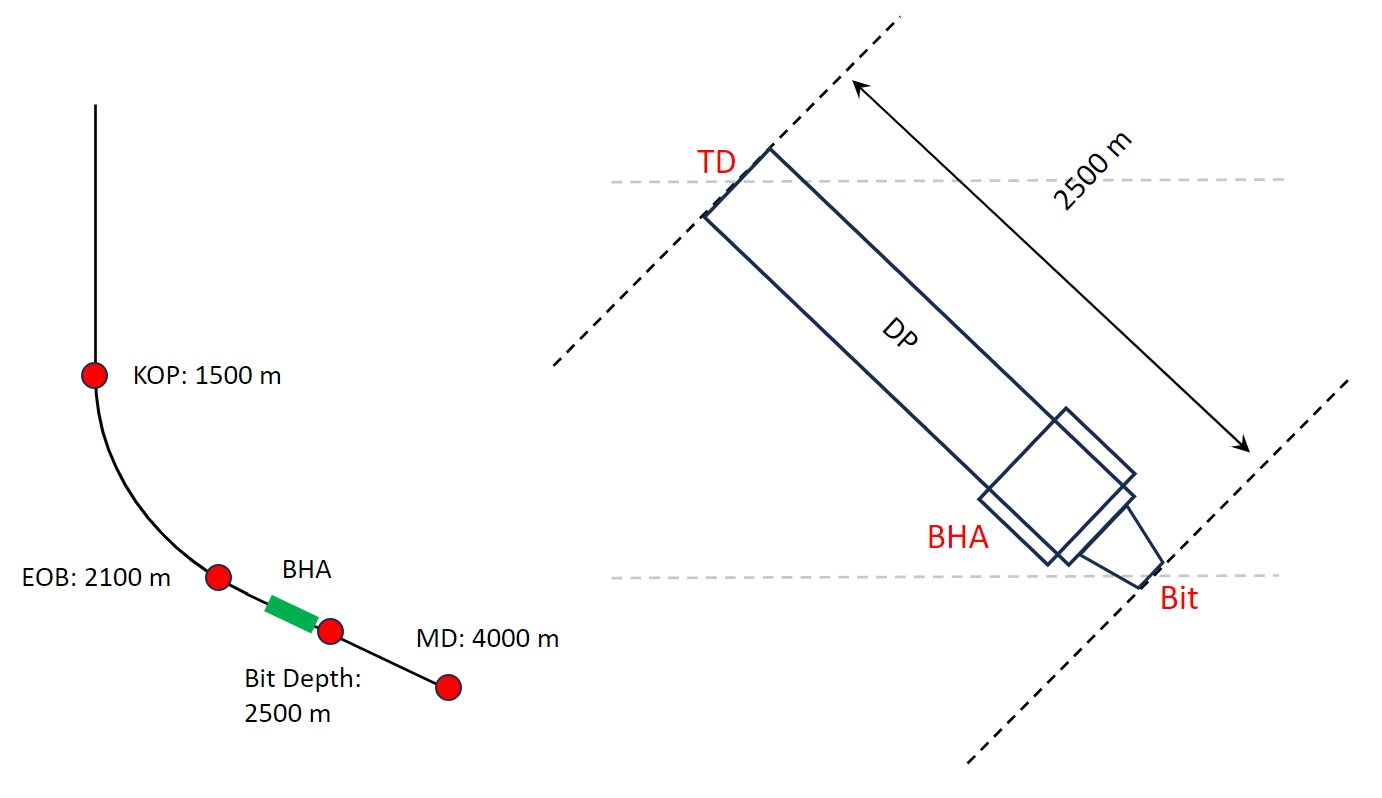
\includegraphics[width=4in]{InclinedWellConfigBHA}
  \caption[Schematic view of Test Case 4]{Schematic view of wellbore and drill string for Test Case 4.}\label{figure_wellconfig_inclined_BHA}
\end{figure}

\begin{table}
    \centering
	\begin{testcasetable}
		$OD_{HWDP}$ & 4.50 $in$ & 0.1143 $m$ & Heavy weight drill pipe outer diameter \\
		\hline
		$ID_{HWDP}$ & 2.50 $in$ & 0.0635 $m$ & Heavy weight drill pipe inner diameter \\
		\hline
		$OD_{DC}$ & 6.00 $in$ & 0.1524 $m$ & Drill collars outer diameter \\
		\hline
		$ID_{DC}$ & 2.00 $in$ & 0.0508 $m$ & Drill collars inner diameter \\
		\hline
		$L_{HWDP}$ & 60 $ft$ & 18.30 $m$ & Length of heavy weight drill pipe \\
		\hline
		$L_{DC}$ & 270 $ft$ & 82.30 $m$ & Length of drill collars \\
		\hline
		$\rho_{dp}$ & 490.6 $lb/ft^3$ & 7850 $kg/m^3$ & Drill pipe density \\
		\hline
		$G_{dp}$ & 1.27$\cdot$10$^{9}$ $lb/ft^2$ & 6.10$\cdot$10$^{10}$ $Pa$ & Drill pipe shear modulus\\
		\hline
		$\mu_{s}$ & 0.5 & 0.5 & Static friction factor\\
		\hline
		$\mu_{d}$ & 0.5 & 0.5 & Dynamic friction factor\\
		\hline
		$w_c$ & 10 $RPM$ & 10 $RPM$ & Cut-off angular velocity\\
		\hline
		$\theta$ & 60$^{\circ}$ & 60$^{\circ}$ & Inclination\\
		\hline
   \end{testcasetable}
   \caption[Input parameters for Test Case 4a]{Input parameters for Test Case 4a, a deviated well with BHA components, and has the same static and dynamic friction factors.}\label{table_Inclinedwell_4a_input}
\end{table}

\subsection{Test Case 4b - Same FF Values}

Lastly, the models were tested with the same configuration as Test Case 4a, except the dynamic friction factor was reduced from 0.5 to 0.25. \tablename~\ref{table_Inclinedwell_4b_input} summarizes the input parameters.

\reviewcomment{Aren't \tablename{}s~\ref{table_Inclinedwell_4a_input} and~\ref{table_Inclinedwell_4b_input} the same?}
\begin{table}
	\centering
	\begin{testcasetable}
		$OD_{HWDP}$ & 4.50 $in$ & 0.1143 $m$ & Heavy weight drill pipe outer diameter \\
		\hline
		$ID_{HWDP}$ & 2.50 $in$ & 0.0635 $m$ & Heavy weight drill pipe inner diameter \\
		\hline
		$OD_{DC}$ & 6.00 $in$ & 0.1524 $m$ & Drill collars outer diameter \\
		\hline
		$ID_{DC}$ & 2.00 $in$ & 0.0508 $m$ & Drill collars inner diameter \\
		\hline
		$L_{HWDP}$ & 60 $ft$ & 18.30 $m$ & Length of heavy weight drill pipe \\
		\hline
		$L_{DC}$ & 270 $ft$ & 82.30 $m$ & Length of drill collars \\
		\hline
		$\rho_{dp}$ & 490.6 $lb/ft^3$ & 7850 $kg/m^3$ & Drill pipe density \\
		\hline
		$G_{dp}$ & 1.27$\cdot$10$^{9}$ $lb/ft^2$ & 6.10$\cdot$10$^{10}$ $Pa$ & Drill pipe shear modulus\\
		\hline
		$\mu_{s}$ & 0.5 & 0.5 & Static friction factor\\
		\hline
		$\mu_{d}$ & 0.25 & 0.25 & Dynamic friction factor\\
		\hline
		$w_c$ & 10 $RPM$ & 10 $RPM$ & Cut-off angular velocity\\
		\hline
		$\theta$ & 60$^{\circ}$ & 60$^{\circ}$ & Inclination\\
		\hline
	\end{testcasetable}
	\caption[Input parameters for Test Case 4b]{Input parameters for Test Case 4b.}\label{table_Inclinedwell_4b_input}
\end{table}
